\documentclass[a4paper,10pt]{article}
\usepackage{listings}
\usepackage{color}
\usepackage{graphicx}
\usepackage{textcomp}

\lstset{language=Java}
\lstset{breaklines=true, numbers=left}
\lstset{tabsize=4}

\definecolor{CommentColor}{rgb}{0,0.5,0} 
\definecolor{KeywordColor}{rgb}{0,0,0.5}

\lstset{commentstyle=\scriptsize\color{CommentColor}\itshape}
\lstset{keywordstyle=\scriptsize\color{KeywordColor}\bfseries}
\lstset{basicstyle=\scriptsize}
\lstset{identifierstyle=\scriptsize}
\lstset{stringstyle=\scriptsize}

% \lstset{basicstyle=\ttfamily}

\definecolor{lightblue}{rgb}{0.7,0.7,1}
\definecolor{lightyellow}{rgb}{1,1,0.5}
\definecolor{lightred}{rgb}{1,0.5,0.5}
\definecolor{lightgreen}{rgb}{0.7,1,0.7}

\newcommand{\src}[1]{\texttt{#1}}

\newcommand{\property}[4]{\item[#1] \mbox{ } \begin{description} \item[Type] \src{#2} \item[Default] #3 \item[Usage] #4  \end{description}}

% thanks to http://www.alfredklomp.com/programming/tex/macros/
\long\def\greybox#1#2#3{%
    \newbox\contentbox%
    \newbox\bkgdbox%
    \setbox\contentbox\hbox to \hsize{%
        \vtop{
            \kern\columnsep
            \hbox to \hsize{%
                \kern\columnsep%
                \advance\hsize by -2\columnsep%
                \parbox{0.1\hsize}{\includegraphics[width=\hsize]{#2}}%
                \hspace{0.025\hsize}%
                \advance\hsize by -0.125\hsize%
                \setlength{\textwidth}{\hsize}%
                \vbox{
                    \parskip=\baselineskip
                    \parindent=0bp
                    \parbox[c]{\hsize}{#3}
                }%
                \kern\columnsep%
            }%
            \kern\columnsep%
        }%
    }%
    \setbox\bkgdbox\vbox{
	\color{#1}
        \hrule width  \wd\contentbox %
               height \ht\contentbox %
               depth  \dp\contentbox
	\color{black}
    }%
    \wd\bkgdbox=0bp%
    \vbox{\hbox to \hsize{\box\bkgdbox\box\contentbox}}%
    \vskip\baselineskip%
}

\newcommand{\designbox}[1]{\greybox{lightgreen}{design}{#1}}
\newcommand{\classbox}[1]{\greybox{lightyellow}{class}{#1}}
\newcommand{\warningbox}[1]{\greybox{lightred}{stop}{#1}}
\newcommand{\infobox}[1]{\greybox{lightblue}{info}{#1}}

\title{DockingFrames 1.0.7 - Common}
\author{Benjamin Sigg}

\begin{document}

\maketitle
\newpage

\tableofcontents
\newpage

\section{Introduction}

\src{DockingFrames} is an open source Java Swing framework. This framework allows to write applications with floating panels. A floating panel is a \src{Component} that can be moved around by the user.

\src{DockingFrames} consists of two libraries, \src{Core} and \src{Common}. \src{Common} provides advanced functionalities that are built on top of \src{Core}. \src{Common} is a wrapper around \src{Core} and requires \src{Core} to work.

This document covers only \src{Common}, \src{Core} has its own guide. Not all the details of \src{Common} are described, but this document gives a nice oversight of the more important aspects.

You can utilize \src{Common} without understanding \src{Core}. But knowing at least some basics about \src{Core} will make life much easier.

\section{Notation}
This document uses various notations.

Any element that can be source code (e.g. a class name) and project names are written mono-spaced like this: \src{java.lang.String}. The package of classes and interfaces is rarely given since almost no name is used twice. The packages can be easily found with the help of the generated API documentation (\src{JavaDoc}).

\infobox{Tips and tricks are listed in boxes.}

\warningbox{Important notes and warnings are listed in boxes like this one.}

\classbox{Implementation details, especially lists of class names, are written in boxes like this.}

\designbox{These boxes explain \textit{why} some thing was designed the way it is. This might either contain some bit of history or an explanation why some awkward design is not as bad as it first looks.}

\section{Basics}
\src{Common} is partitioned into three sub-projects.

For clients the sub-project \src{common} is the most interesting. This project is the main layer above \src{Core} and also the most advanced layer in the whole framework.

The sub-project \src{facile} builds a basis for the features of \src{common}. In theory \src{facile} could be used without \src{common} but in practice the classes and interfaces are clearly designed to be used by or together with \src{common}.

Finally \src{support} consists of classes that are just used by \src{facile} and \src{common}. These classes have few to none relations with \src{DockingFrames} and can be used alone as well.

\section{Concepts}
In the understanding of \src{Common} an application consists of one main-frame and maybe several supportive frames and dialogs. The main-frame is a \src{JFrame} and the application runs as long as this frame is visible. The main-frame consists of several panels. Each panel shows some part of the data. E.g. the panels of a browser could be the ``history'', the ``bookmarks'' and the open websites.

\src{Common} is an additional layer between panels and main-frame. It separates them and allows the user to drag \& drop panels.

\begin{figure}[ht]
\centering
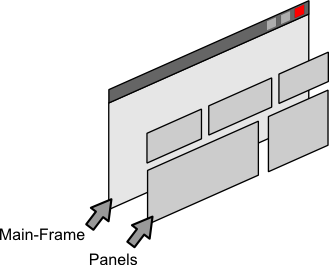
\includegraphics[scale=1]{app_without}
\caption{The standard application without \src{Common}. A main-frame and some panels that are put onto the main-frame.}
\label{fig:app_without}
\end{figure}

\begin{figure}[ht]
\centering
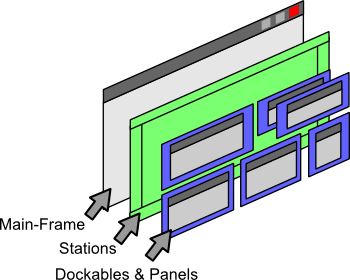
\includegraphics[scale=1]{app_with}
\caption{An application with \src{Common}. The panels are wrapped into dockables. The dockables are put onto stations which lay on the main-frame. Dockables can be moved to different stations.}
\label{fig:app_with}
\end{figure}

\end{document}